\documentclass[]{article}
\usepackage{lmodern}
\usepackage{setspace}
\setstretch{1.5}
\usepackage{amssymb,amsmath}
\usepackage{ifxetex,ifluatex}
\usepackage{fixltx2e} % provides \textsubscript
\ifnum 0\ifxetex 1\fi\ifluatex 1\fi=0 % if pdftex
  \usepackage[T1]{fontenc}
  \usepackage[utf8]{inputenc}
\else % if luatex or xelatex
  \ifxetex
    \usepackage{mathspec}
  \else
    \usepackage{fontspec}
  \fi
  \defaultfontfeatures{Ligatures=TeX,Scale=MatchLowercase}
\fi
% use upquote if available, for straight quotes in verbatim environments
\IfFileExists{upquote.sty}{\usepackage{upquote}}{}
% use microtype if available
\IfFileExists{microtype.sty}{%
\usepackage{microtype}
\UseMicrotypeSet[protrusion]{basicmath} % disable protrusion for tt fonts
}{}
\usepackage[margin=1in]{geometry}
\usepackage{hyperref}
\hypersetup{unicode=true,
            pdftitle={iDADwigl - a R package for open-system uranium-thorium dating},
            pdfauthor={Anthony Dosseto\^{}1\^{},\^{}* and Ben Marwick\^{}2},
            pdfborder={0 0 0},
            breaklinks=true}
\urlstyle{same}  % don't use monospace font for urls
\usepackage{graphicx,grffile}
\makeatletter
\def\maxwidth{\ifdim\Gin@nat@width>\linewidth\linewidth\else\Gin@nat@width\fi}
\def\maxheight{\ifdim\Gin@nat@height>\textheight\textheight\else\Gin@nat@height\fi}
\makeatother
% Scale images if necessary, so that they will not overflow the page
% margins by default, and it is still possible to overwrite the defaults
% using explicit options in \includegraphics[width, height, ...]{}
\setkeys{Gin}{width=\maxwidth,height=\maxheight,keepaspectratio}
\IfFileExists{parskip.sty}{%
\usepackage{parskip}
}{% else
\setlength{\parindent}{0pt}
\setlength{\parskip}{6pt plus 2pt minus 1pt}
}
\setlength{\emergencystretch}{3em}  % prevent overfull lines
\providecommand{\tightlist}{%
  \setlength{\itemsep}{0pt}\setlength{\parskip}{0pt}}
\setcounter{secnumdepth}{0}
% Redefines (sub)paragraphs to behave more like sections
\ifx\paragraph\undefined\else
\let\oldparagraph\paragraph
\renewcommand{\paragraph}[1]{\oldparagraph{#1}\mbox{}}
\fi
\ifx\subparagraph\undefined\else
\let\oldsubparagraph\subparagraph
\renewcommand{\subparagraph}[1]{\oldsubparagraph{#1}\mbox{}}
\fi

%%% Use protect on footnotes to avoid problems with footnotes in titles
\let\rmarkdownfootnote\footnote%
\def\footnote{\protect\rmarkdownfootnote}

%%% Change title format to be more compact
\usepackage{titling}

% Create subtitle command for use in maketitle
\newcommand{\subtitle}[1]{
  \posttitle{
    \begin{center}\large#1\end{center}
    }
}

\setlength{\droptitle}{-2em}

  \title{iDADwigl - a R package for open-system uranium-thorium dating}
    \pretitle{\vspace{\droptitle}\centering\huge}
  \posttitle{\par}
    \author{Anthony Dosseto\(^1\)\(^,\)\(^*\) and Ben Marwick\(^2\)}
    \preauthor{\centering\large\emph}
  \postauthor{\par}
    \date{}
    \predate{}\postdate{}
  
\usepackage[format=plain,labelsep=period,textformat=period,justification=justified,singlelinecheck=false]{caption} % package to align left captions
\usepackage{colortbl} % to be able to use kableExtra package with latex
\usepackage{lineno} % package for line numbers
\usepackage{floatrow} % package needed to align left tables
\usepackage{pdflscape} % package to show landscape orientation

% commands to enter and exit landscape orientation
\newcommand{\blandscape}{\begin{landscape}}
\newcommand{\elandscape}{\end{landscape}}

% to align left tables
\floatsetup[table]{style=ruled,
  objectset=raggedright,
  margins=raggedright,
  midcode=captionskip,
  captionskip=10pt}

\begin{document}
\maketitle

\(^1\)Wollongong Isotope Geochronology Laboratory, School of Earth \&
Envrionmental Sciences. University of Wollongong. Wollongong NSW
Australia

\(^2\)Ben's affiliation

\(^*\)Corresponding author:
\href{mailto:tonyd@uow.edu.au}{\nolinkurl{tonyd@uow.edu.au}}

\newpage
\linenumbers

\hypertarget{introduction}{%
\section{Introduction}\label{introduction}}

Open-system uranium-thorium (U-Th) dating of teeth and bones, while
challenging, has revolutionised our ability to provide reliable
chronology for humans and fauna (Eggins et al., 2005; Sambridge et al.,
2012; Grün et al., 2014). Thus, this approach has significantly improved
our understanding of human evolution (e.g. Dirks et al., 2017; Sutikna
et al., 2016). Uranium-thorium dating is based on the premise that a
material takes up U but no Th, so all the \textsuperscript{230}Th in the
sample comes from decay of \textsuperscript{238}U. If detrital Th is
included to the sample, a correction must be included to account for the
fraction of \textsuperscript{230}Th which is detrital and not derived
from \textsuperscript{238}U decay. Another requirement is that there is
no gain or loss of \textsuperscript{230}Th, \textsuperscript{234}U or
\textsuperscript{238}U after formation of the material. While it is
often the case for many geological samples such as corals or
speleothems, this requirement is rarely met for teeth and bone (although
enamel can sometimes be quite impervious to isotope gain or loss). Thus,
for teeth and bone, U-Th dating requires to take into account open
system behaviour. The diffusion-adsorption-decay model developed by
Sambridge et al. (2012) was instrumental to implement successfully
open-system U-Th dating. It allows for advective and diffusive transport
of uranium and thorium isotopes, while include synchronous radioactive
decay. The software implementation was written in Fortran and is
available as a Java GUI (\url{http://www.iearth.org.au/codes/iDaD/}). In
this article, we propose a R package which implements the model of
Sambridge et al. (2012).

\hypertarget{methods}{%
\section{Methods}\label{methods}}

Data required for the DAD model are
(\textsuperscript{230}Th/\textsuperscript{238}U) and
(\textsuperscript{234}U/\textsuperscript{238}U) activity ratios
collected along a transect perpendicular to the surface of the tooth or
bone (brackets denote activity ratios throughout this article). Sampling
for analysis can be done by micro-drilling or laser ablation. If the
former, aliquots are then dissolved, followed by separation of U and Th
using ion exchange chromatography. This is more time consuming (at least
one week of work) than laser ablation, where the material sampled by the
laser is directly sent to the mass spectrometer. While laser ablation
also offers a better spatial resolution than micro-drilling, the
precision of the data is inferior because of the much smaller amount of
material sampled. Uranium and thorium isotope ratios are then analysed
by multi-collector inductively-coupled plasma mass spectrometry. A
plasma ionise all U and Th atoms, their isotopes are separated through a
magnetic field and each collected in a different collector. If using
laser ablation, it is best to have two ion counters so
\textsuperscript{230}Th and \textsuperscript{234}U can be collected
simultaneously.\\
The distance of each analysis location from the inner and outer surfaces
of the bones, for instance, needs to be recorded. One surface is given a
coordinate of 1 and the other one -1, thus coordinates of analyses take
values in between (Fig. 1). The script requires a csv file with the
following columns: \emph{iDAD position}, \emph{U234\_U238\_CORR},
\emph{U234\_U238\_CORR\_Int2SE}, \emph{iDAD position},
\emph{Th230\_U238\_CORR}, \emph{Th230\_U238\_CORR\_Int2SE},
\emph{U\_ppm} and \emph{U\_ppm\_Int2SE}. The R package comes with two
examples of input files. The first \emph{iDAD position} column
corresponds to the coordinates of the
(\textsuperscript{234}U/\textsuperscript{238}U) analyses, which as
indicated above take values between -1 and 1. The second \emph{iDAD
position} column is used if the coordinates of the
(\textsuperscript{230}Th/\textsuperscript{238}U) analyses are different
from those of the (\textsuperscript{234}U/\textsuperscript{238}U)
analyses. Columns \emph{U234\_U238\_CORR} and
\emph{U234\_U238\_CORR\_Int2SE} are the
(\textsuperscript{234}U/\textsuperscript{238}U) activity ratios and
their 2\(\sigma\) errors. Columns \emph{Th230\_U238\_CORR} and
\emph{Th230\_U238\_CORR\_Int2SE} are the
(\textsuperscript{230}Th/\textsuperscript{238}U) activity ratios and
their 2\(\sigma\) errors. Columns \emph{U\_ppm} and
\emph{U\_ppm\_Int2SE} and calculated uranium concentrations (in ppm) and
their 2\(\sigma\) errors. Uranium concentrations are not necessary for
the model and only used for display of the U concentration profile in a
figure.

\begin{figure}
\centering
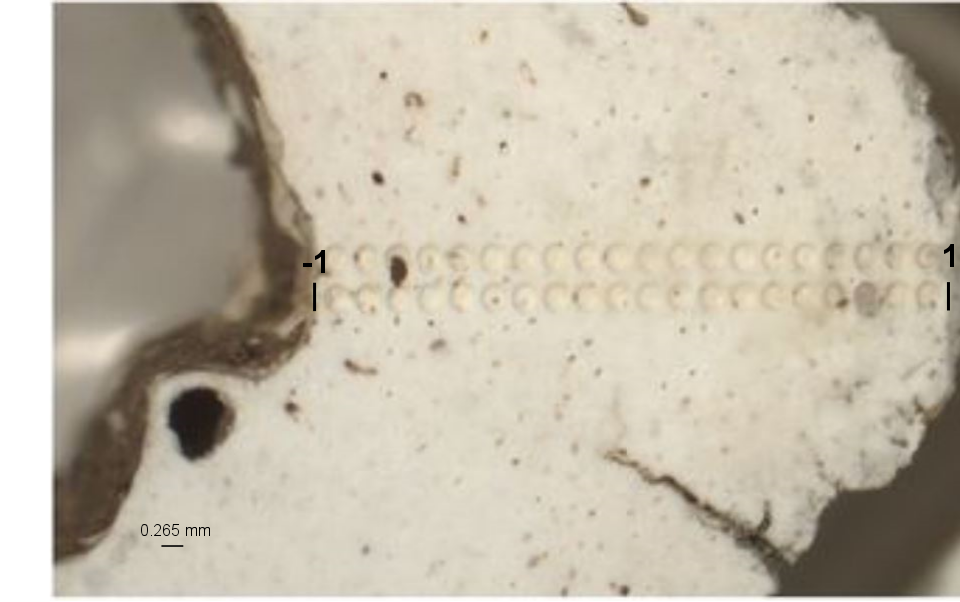
\includegraphics{input/bone.png}
\caption{Modern human femur (132A/LB/27D/03) from Liang Bua, Flores,
Indonesia. Two analysis transects can be seen. For a given transect, the
outer and inner surface of the bone are given 1 and -1 reference
coordinates, and the position of each analysis is calculated
accordingly. Modified from Sutikna et al. (2016)}
\end{figure}

\hypertarget{running-the-script}{%
\section{Running the script}\label{running-the-script}}

In the folder where you store the R script \emph{run\_this}, create two
folders on your computer named ``input'' and ``output''. In the
``input'' folder, place the csv file(s) in the ``input'' folder. Open
the \emph{run\_this} script. For \emph{path\_wd}, enter the full path
where your R scripts are. For \emph{input\_file\_name}, enter the name
of the data file. For \emph{sample\_name}, enter the chosen sample name
you want to display on figures. \emph{nbit} is the number of iterations.
For the first run, set to 1. \emph{fsum\_target} is the sum of the
squared differences between the calculated and observed activity ratios.
Give it a low value to start with (e.g.~0.05). For \emph{l}, enter the
thickness of the sample (in cm). For instance, for the modern human
bone, thickness is 5.35 cm. For \emph{U\_0}, enter the U concentration
at the surface (in ppm). This value does not significantly affect the
model results and values from analyses near either surface of the sample
can be used as a guide. \emph{K\_min} and \emph{K\_max} are the minimum
and maximum values allowed for the uranium diffusion coefficient (in
cm\textsuperscript{2}/s). Values between 10\textsuperscript{-13} and
10\textsuperscript{-11} cm\textsuperscript{2}/s are generally
appropriate. \emph{U48\_0\_min} and \emph{U48\_0\_max} are the minimum
and maximum values allowed for the
(\textsuperscript{234}U/\textsuperscript{238}U) activity ratio at the
surface of the sample. Since
(\textsuperscript{234}U/\textsuperscript{238}U) does not vary greatly
over the time period generally studied, the values measured near the
surface of the sample can be used as a guide. These values can be
adjusted if the model fit to the data is not optimal. \emph{T\_min} and
\emph{T\_max} are minimum and maximum values allowed for the age (in
yr). If there is no estimated knowledge of the sample age, the range of
values can be 1,000 to 500,000 yr and adjusted later.

Run the script \emph{run\_this} by pressing ``Source'' in R studio. This
will generate figures with the U concentration profile, the observed and
calculated (\textsuperscript{234}U/\textsuperscript{238}U) activity
ratios and the observed and calculated
(\textsuperscript{230}Th/\textsuperscript{238}U) activity ratios. The
model calculated age and (\textsuperscript{234}U/\textsuperscript{238}U)
ratio at the surface are also saved in a csv file named with the sample
name and the mention ``model\_results''. Error reported in this file are
the 67\% and 33\% quantiles. The sample age is in years before the date
of analysis. The calculated activity ratios are also saved in a separate
csv file named with the sample name and the mention ``calc\_ratios''.
The environment is also saved in a Rdata file with the sample name. The
model age is also displayed in the console with its error reported as
the 67\% and 33\% quantiles.

Optimise the fit by change the range of allowed values for the
(\textsuperscript{234}U/\textsuperscript{238}U) ratio at the surface and
the age of the sample, and by decreasing the \emph{fsum\_target}. Once
you obtain a satisfying fit (by visual inspection of the produced
figures), increase \emph{nbit} to a higher value (e.g.~1000) and run the
model again.

\hypertarget{test-results}{%
\section{Test results}\label{test-results}}

The package is provided with two sample data sets derived from Sutikna
et al. (2016): ``Hobbit\_MH2T\_for\_iDAD.csv'' is data from transect 2
for modern human femur 132A/LB/27D/03. ``Hobbit\_1-1T\_for\_iDAD.csv''
is data from transect 1 for \emph{Homo floresiensis} ulna LB1/52. For
the latter, six analyses were removed from the set as in (Sutikna et
al., 2016). For transect 2 of 132A/LB/27D/03, Sutikna et al. (2016)
reported an age of 7.4 \(\pm\) 0.5 ka (thousand years before 2014). With
iDADwigl, we obtain an age of 7.1 +0.6/-0.7 ka (Figs. 2-4). For transect
1 of LB1/52, Sutikna et al. (2016) reported an age of 79.0 \(\pm\) 3.7
ka. With iDADwigl, we obtain an age of 75.4 \(\pm\) 0.9 ka.

\begin{figure}
\centering
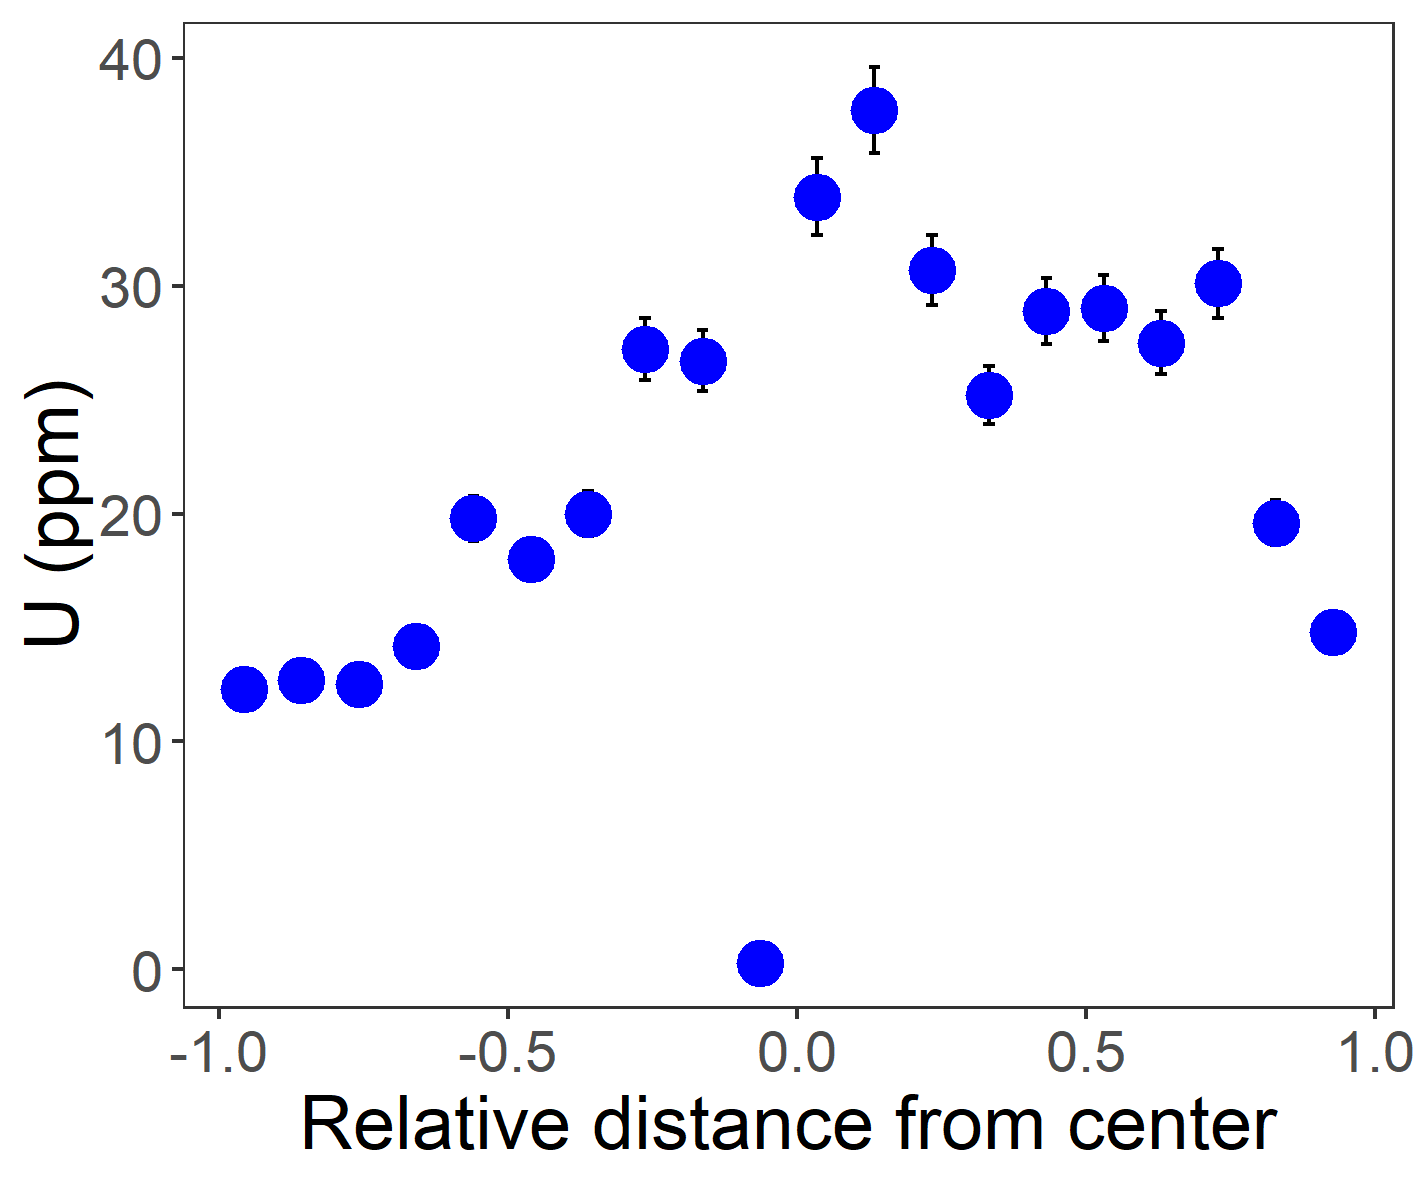
\includegraphics{input/U_Hobbit_MH2T_DAD.png}
\caption{Uranium concentration profile for transect 2 of modern human
femur 132A/LB/27D/03}
\end{figure}

\begin{figure}
\centering
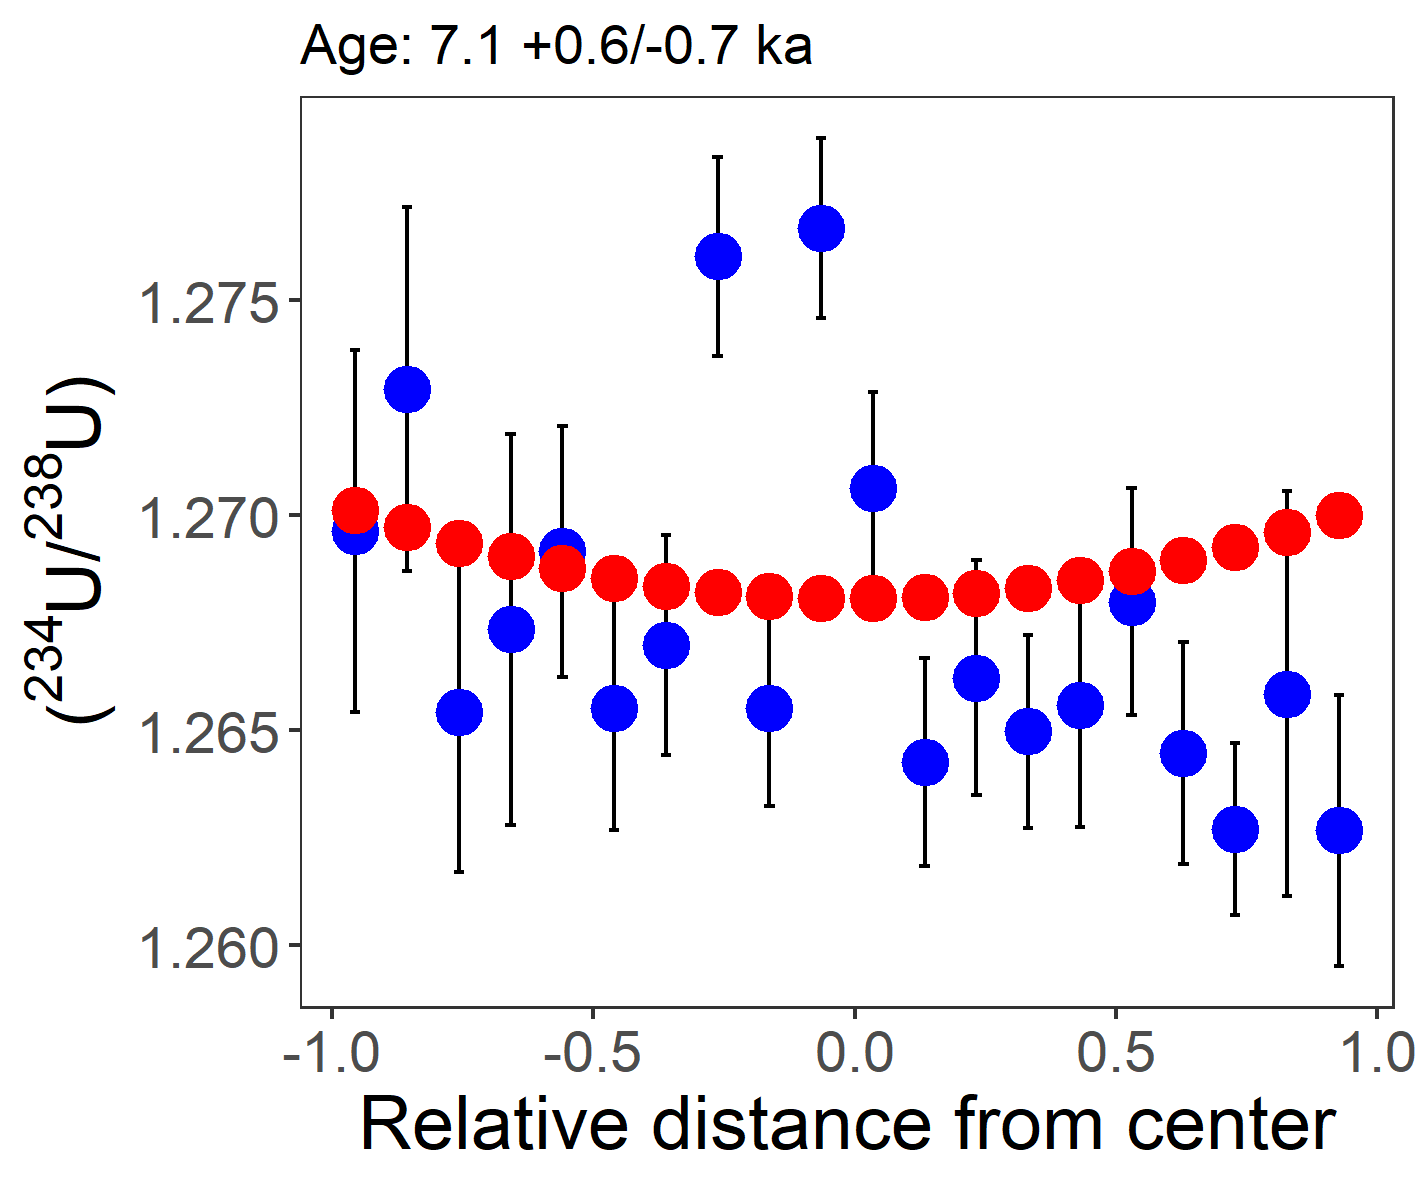
\includegraphics{input/R48_Hobbit_MH2T_DAD.png}
\caption{Calculated (red) and observed (blue)
(\textsuperscript{234}U/\textsuperscript{238}U) activity ratios for
transect 2 of modern human femur 132A/LB/27D/03.}
\end{figure}

\begin{figure}
\centering
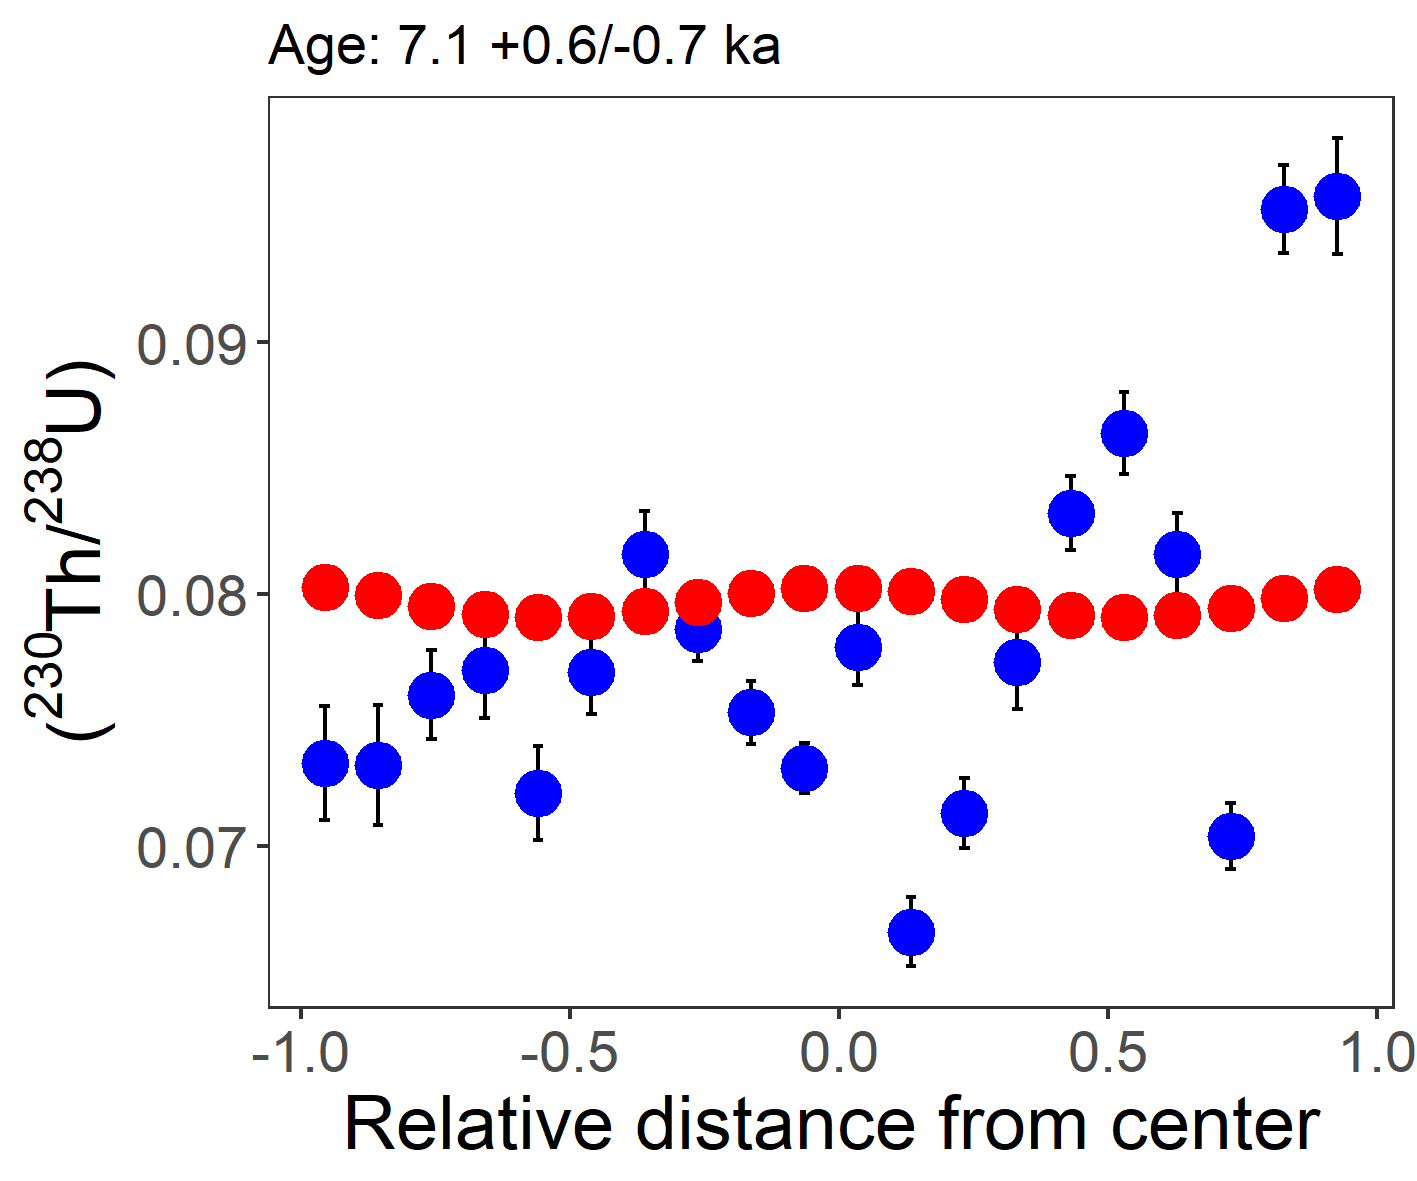
\includegraphics{input/R08_Hobbit_MH2T_DAD.png}
\caption{Calculated (red) and observed (blue)
(\textsuperscript{230}Th/\textsuperscript{238}U) activity ratios for
transect 2 of modern human femur 132A/LB/27D/03}
\end{figure}

\newpage
\nolinenumbers

\hypertarget{references}{%
\section*{References}\label{references}}
\addcontentsline{toc}{section}{References}

\hypertarget{refs}{}
\leavevmode\hypertarget{ref-Dirks2017}{}%
Dirks P. H., Roberts E. M., Hilbert-Wolf H., Kramers J. D., Hawks J.,
Dosseto A., Duval M., Elliott M., Evans M., Grun R., Hellstrom J.,
Herries A. I., Joannes-Boyau R., Makhubela T. V., Placzek C. J., Robbins
J., Spandler C., Wiersma J., Woodhead J. and Berger L. R. (2017) The age
of homo naledi and associated sediments in the rising star cave, south
africa. \emph{Elife} \textbf{6}. Available at:
\url{https://www.ncbi.nlm.nih.gov/pubmed/28483040}.

\leavevmode\hypertarget{ref-Eggins2005}{}%
Eggins S. M., Grün R., McCulloch M. T., Pike A. W. G., Chappell J.,
Kinsley L., Mortimer G., Shelley M., Murray-Wallace C. V., Spötl C. and
Taylor L. (2005) In situ u-series dating by laser-ablation
multi-collector icpms: New prospects for quaternary geochronology.
\emph{Quaternary Science Reviews} \textbf{24}, 2523--2538.

\leavevmode\hypertarget{ref-Gruen2014}{}%
Grün R., Eggins S., Kinsley L., Moseley H. and Sambridge M. (2014) Laser
ablation u-series analysis of fossil bones and teeth.
\emph{Palaeogeography, Palaeoclimatology, Palaeoecology} \textbf{416},
150--167. Available at:
\url{http://www.sciencedirect.com/science/article/pii/S0031018214003782}.

\leavevmode\hypertarget{ref-Sambridge2012}{}%
Sambridge M., Grün R. and Eggins S. (2012) U-series dating of bone in an
open system: The diffusion-adsorption-decay model. \emph{Quaternary
Geochronology}. Available at:
\url{http://www.scopus.com/inward/record.url?eid=2-s2.0-84857958926\&partnerID=40\&md5=01e7f1b7d3554da26b247125425ff496}.

\leavevmode\hypertarget{ref-Sutikna2016}{}%
Sutikna T., Tocheri M. W., Morwood M. J., Saptomo E. W., Jatmiko, Awe R.
D., Wasisto S., Westaway K. E., Aubert M., Li B., Zhao J.-x., Storey M.,
Alloway B. V., Morley M. W., Meijer H. J. M., Bergh G. D. van den, Grün
R., Dosseto A., Brumm A., Jungers W. L. and Roberts R. G. (2016) Revised
stratigraphy and chronology for homo floresiensis at liang bua in
indonesia. \emph{Nature} \textbf{532}, 366--369. Available at:
\url{http://dx.doi.org/10.1038/nature17179}.


\end{document}
